\section*{\nr.3 \titthree (10 Punkte)}
\begin{enumerate}[(a)]
\item Das elektrische Feld ergibt sich aus der Überlagerung der beiden Felder der beiden Punktladungen. Diese erzeugen jeweils ein Feld von
\begin{equation}
  \vec E_+(\vec r)= \frac{1}{4 \pi \epsilon_0}\frac{q}{|\vec r - \vec r_1|^3}(\vec r - \vec r_1)
\end{equation}
und
\begin{equation}
  \vec E_-(\vec r)= \frac{1}{4 \pi \epsilon_0}\frac{-q}{|\vec r - \vec r_2|^3}(\vec r - \vec r_2),
\end{equation}
was mit der Definition des Koordinatenursprungs in der Mitte zwischen den beiden Ladungen ein Gesamtfeld von
\begin{align}
  \vec E(\vec r) &= \frac{q}{4 \pi \epsilon_0}\left(\frac{(\vec r - \vec r_1)}{|\vec r - \vec r_1|^3}-\frac{(\vec r - \vec r_2)}{|\vec r - \vec r_2|^3}\right) \\  
  &= \frac{q}{4 \pi \epsilon_0}\left(\frac{\left(\begin{pmatrix} x\\y \end{pmatrix} - \begin{pmatrix} a\\0 \end{pmatrix}\right)}{|(x-a)^2+y^2|^{\frac{3}{2}}}-\frac{\left(\begin{pmatrix} x\\y \end{pmatrix} + \begin{pmatrix} a\\0 \end{pmatrix}\right)}{|(x+a)^2+y^2)|^{\frac{3}{2}}}\right)
\end{align}
ergibt.

\item Skizze:

    \begin{figure}[H]
    \begin{center}
    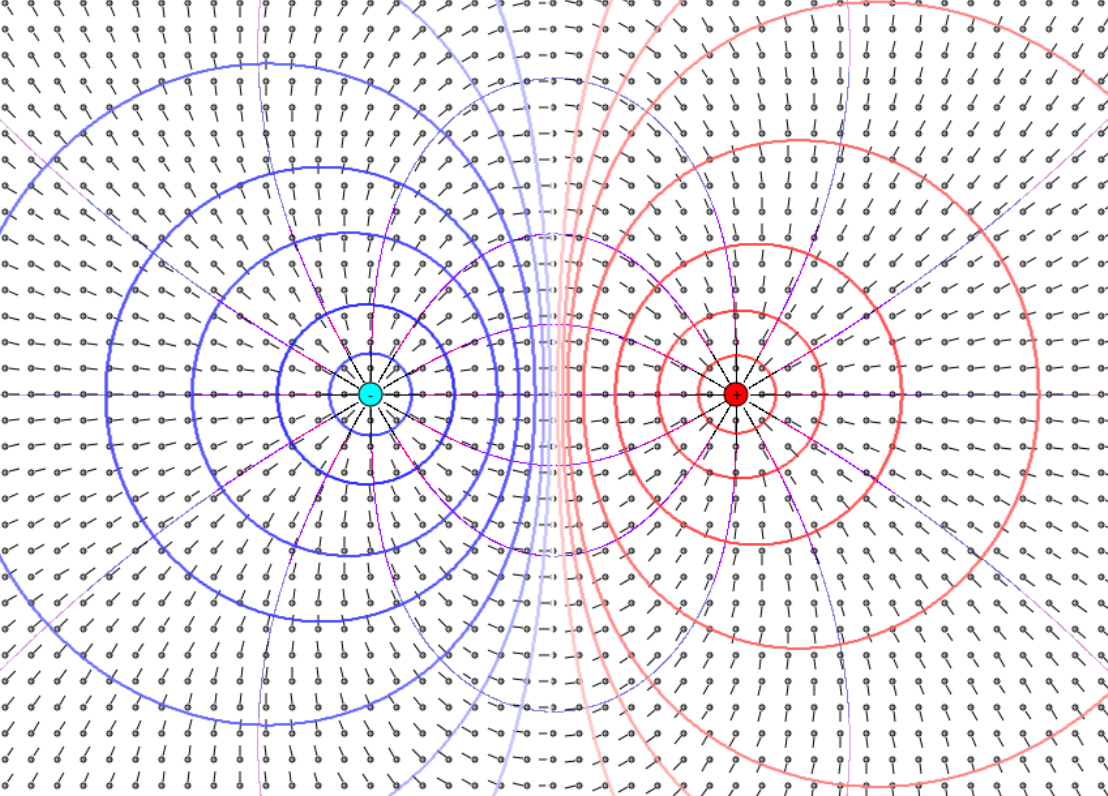
\includegraphics[width=0.6\textwidth]{Aufgaben/Skizze.png}
    \caption{Skizze der Feldlinien sowie Äquipotentiallinien}
    \label{f:times}
    \end{center}
    \end{figure}

\item Auf der x-Achse gilt
\begin{align}
  \vec E(x) &= \frac{q}{4 \pi \epsilon_0}\left(\frac{(x-a)}{|x-a|^3}-\frac{(x+a)}{|x+a|^3}\right)\vec e_x\\
  &=\frac{q}{4 \pi \epsilon_0}\left(\frac{1}{(x-a)^2}-\frac{1}{(x+a)^2}\right)\vec e_x\\
  &=\frac{q}{4 \pi \epsilon_0}\left(\frac{4ax}{(a^2-x^2)^2}\right)\vec e_x\\
  &=\frac{p}{2 \pi \epsilon_0}\left(\frac{x}{(a^2-x^2)^2}\right)\vec e_x\\
  &\approx\frac{p}{2 \pi \epsilon_0}\frac{x}{x^4}\vec e_x\\
  &=\frac{p}{2 \pi \epsilon_0}\frac{1}{x^3}\vec e_x
\end{align}

\item Auf der y-Achse gilt
\begin{align}
\vec E(y) &= \frac{q}{4 \pi \epsilon_0}\left(\frac{\begin{pmatrix} -a\\y \end{pmatrix}}{(a^2+y^2)^{\frac{3}{2}}}-\frac{\begin{pmatrix} a\\y \end{pmatrix}}{(a^2+y^2)^{\frac{3}{2}}}\right)\\
 &= \frac{q}{4 \pi \epsilon_0}\frac{-2a}{(a^2+y^2)^{\frac{3}{2}}} \vec e_x\\
 &= \frac{-p}{4 \pi \epsilon_0}\frac{1}{(a^2+y^2)^{\frac{3}{2}}} \vec e_x\\
 &\approx \frac{-p}{4 \pi \epsilon_0}\frac{1}{y^3} \vec e_x
\end{align}

\end{enumerate}